\chapter{基于核密度估计的时空路网数据可视化}
\label{sec3:paper1}

\section{问题定义及已有最优算法}
\label{sec3:preliminaries}

\subsection{问题定义}

首先,我们给出TN-KDE问题的形式化定义以及已有的最优算法。本章节所用到的主要符号含义已列在表~\ref{tab:symbols} 中。

\begin{table}[h]
	\centering
	\def\arraystretch{1.5}
	\caption{主要符号及对应描述}
	\label{tab:symbols}
	\begin{tabular}{l|l}
	\hline
	符号  & 描述 \\ \hline\hline
	$G=(V,E)$      & 图 $G$,包括点集 $V$ 和边集 $E$ \\
	$q$	     	   & 查询的线段点 \\
	$t$		       & 查询的时间 \\
	$o_i = (p_i, t_i)$ & 数据点 $o_i$,包括位置 $p_i$ 和时间 $t_i$ \\
	$d(u, v)$      & 点 $u$ 到 $v$ 的最短路径距离 \\
	$b_s, b_t$     & 空间和时间维度上的带宽范围 \\
	$L, N$		   & 线段点和数据点的总数 \\
	$n_e$          & 边 $e$ 上的数据点 \\
	\hline
	\end{tabular}
\end{table}

\begin{definition}[路网图]
一个路网图可以被形式化地定义为图 $G = (V, E)$,其中 $V$ 和 $E \subseteq V \times V$ 分别是点集和边集。任意两点 $v_a$ 和 $v_b$ 的距离 $d(v_a, v_b)$ 被定义为两点间的最短路径距离。
\end{definition}

为了计算路网图上的核密度,我们根据已有的常见处理方式~\cite{xie_kernel_2008, chan_fast_2021}将每条边均匀分成若干相同长度的小段,称为线段点(Linear Pixel,Lixel)。和平面核密度计算中的像素点类似,每个线段点都需要执行一次核密度的计算,并且使用该线段点的中点作为度量距离的位置。

\begin{figure}[h]\centering
	\scalebox{0.7}[0.7]{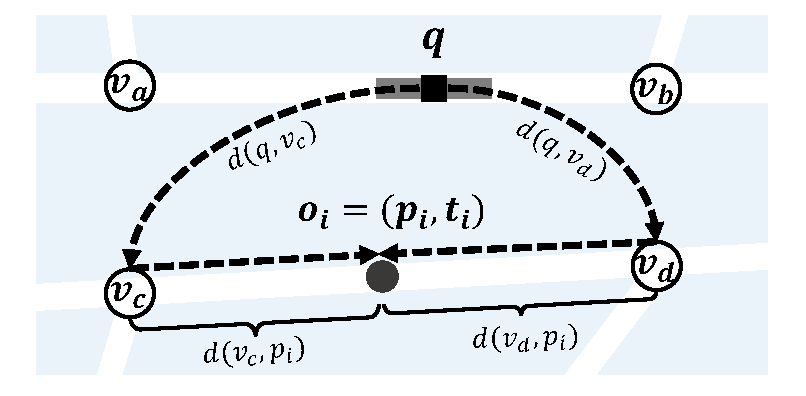
\includegraphics{./figures/sec1_intro.pdf}}
	\caption{线段点$q$(灰色线段)和数据点$o_i$(黑色圆点)的可视化示例。}
	\label{fig:sketch}
\end{figure}


\begin{definition}[线段点]
	给定一个路网图 $G = (V, E)$, 每条边 $(v_a,v_b) \in E$ 都会被分成若干长度相同的线段点,其中距离间隔为 $g$,最后不足 $g$ 的部分会被单独作为一个线段点。在计算最短路径距离时,使用线段点的中点作为计算位置。
\end{definition}

根据该定义,总共的像素点个数为:

\begin{equation*}
	L = \sum_{(v_a,v_b) \in E} \left\lceil \frac{d(v_a,v_b)}{g} \right\rceil
\end{equation*}

同理,数据点的定义如下:
\begin{definition}[数据点]
	一个数据点 $o_i=(p_i, t_i) \in O$ 表示在位置 $p_i$ 和时间 $t_i$ 发生事件。边 $e$ 上的总数据点个数为 $n_e$。图上所有数据点的总数为:
	\begin{equation*}
		N = \sum_{e \in E} n_e
	\end{equation*}
\end{definition}


图~\ref{fig:sketch} 简单展示了这些定义。$q$ 是边 $(v_a, v_b)$ 上的一个线段点,用灰色线段表示,其中心用黑色方块标出。$o_i$ 是边 $(v_c, v_d)$ 上的数据点,用黑色圆点标出。

TN-KDE问题是给定查询的时间和空间带宽范围,在路网图上计算核密度:
\begin{definition}{时空路网核密度估计(Temporal Network Kernel Density Estimation,TN-KDE)}
	给定一个路网图 $G=(V, E)$,一个数据点集合 $O$,空间带宽范围 $b_s$ 和时间带宽范围 $b_t$,TN-KDE问题是计算所有线段点的核密度 $F(q)$:
\begin{equation}
\label{eq-def}
\begin{aligned}
	F(q) &= \sum_{o_i=(p_i, t_i) \in O} f(q, o_i), \\
	f(q, o_i) &= 
	K_s\left(\frac{d(q, p_i)}{b_s}\right)
	K_t\left(\frac{\vert t - t_i \vert}{b_t}\right),
\end{aligned}
\end{equation}
其中 $K_s(\cdot)$ 和 $K_t(\cdot)$ 是核密度函数,可以从表~\ref{tab1}中任意选取。空间距离是最短路径距离$d(d, p_i)$,时间距离为时间差 $\vert t - t_i \vert$。由于核函数的定义域为 $[0,1]$,在带宽范围之外的数据点不会被纳入计算,即只考虑最短路径距离不超过 $b_s$,且发生在时间窗口 $[t - b_t, t + b_t]$ 内的数据点。当所有的线段点都根据该定义计算后,使用放缩因子 $w$ 统一放缩后即可得到热力图(类似于图~\ref{fig:temporal_heatmap})。
\end{definition}

% A TN-KDE query only considers the events with shortest distances less than $b_s$ and time differences less than $b_t$.




\subsection{已有的最优算法}
\label{sec:sota}

根据我们广泛的调研,目前针对路网图上的核密度计算的最优算法为聚合距离增强算法(Aggregate Distance Augmentation,ADA)~\cite{chan_fast_2021}。由于ADA算法仅支持空间距离,不支持时间距离,我们忽略时间核函数并采用Epanechnikov核函数作为空间核函数作为示例,即:
\begin{equation*}
	f(q, o_i) = 1 - \frac{1}{b_s^2} dist(q, p_i)^2
\end{equation*}

ADA算法的第一个关键步骤是将所有数据点以边为单位计算核密度:
The core step of ADA is to rewrite Equation~\ref{eq-def} as:
\begin{equation*}
\label{eq-transform}
\begin{aligned}
	F(q) &= \sum_{e \in E} F_e(q) \\
	F_e(q) &= \sum_{o_i \in O_e} 1 - \frac{1}{b_s^2} d(q, p_i)^2
\end{aligned}
\end{equation*}
其中 $O_e$ 包含所有在边 $e$ 上的数据点。该公式只是重新定义了核密度的计算顺序,并没有改变计算复杂度,但之后我们可以仅专注于计算一条边上的数据点所产生的贡献,即 $F_e(q)$。

\begin{figure}[h]\centering
	\scalebox{0.7}[0.7]{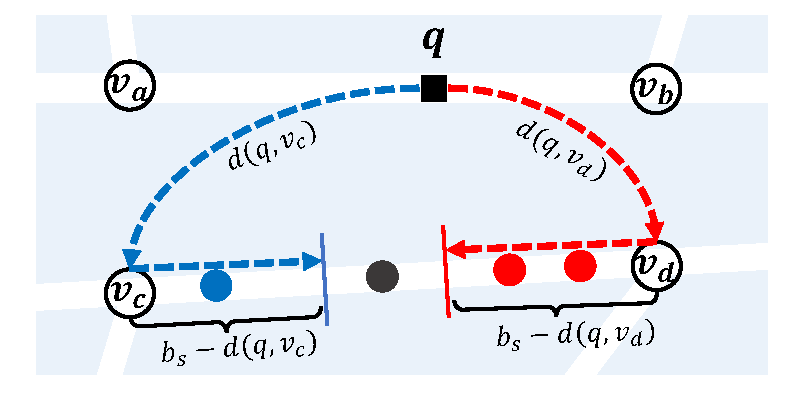
\includegraphics{./figures/Preliminary_ADA.pdf}}
	\caption{ADA算法示例。}
	\label{fig-ADA}
\end{figure}

图~\ref{fig-ADA} 展示了ADA算法的主要思路,这里我们计算边 $(v_c, v_d)$ 上的数据点对线段点 $q$ 的核密度贡献。注意到 $q$ 到所有数据点的位置 $p_i$ 的最短路径一定会通过 $v_c$ 和 $v_d$,此时最短路径分为两种情况:
\begin{itemize}
	\item $q \rightarrow v_c \rightarrow p_i$。此时的最短路径长度为 $d(q, v_c) + d(v_c, p_i)$。
	\item $q \rightarrow v_d \rightarrow p_i$。此时的最短路径长度为 $d(q, v_d) + d(v_d, p_i)$。
\end{itemize}
显然选择第一种路径的数据点一定更靠近 $v_c$(用蓝色表示),而选择第二种路径的数据点一定更靠近 $v_d$(用红色表示)。对于第一种情况来说,这些数据点对核密度的贡献可以表示为:
\begin{equation*}
\begin{aligned}
	F_\Gamma(q) &= \sum_{o_i \in O_\Gamma} \left(1 - \frac{[d(q, v_c) + d(v_c, p_i)]^2}{b_s^2}\right) \\
	% &= \sum_{o_i \in O_\Gamma} \left(1 - \frac{d(q, v_c)^2 + 2d(q, v_c)d(v_c, p_i)+d(v_c,p_i)^2}{b_s^2}\right) \\
	&= \frac{1}{b_s^2} \cdot
	\begin{bmatrix}
		-1 \\
		-2 \cdot d(q, v_c) \\
		b_s^2 - d(q, v_c)^2
	\end{bmatrix}^\top
	\begin{bmatrix}
		\sum_{o_i \in O_\Gamma} d(v_c, p_i)^2 \\
		\sum_{o_i \in O_\Gamma} d(v_c, p_i) \\
		\vert O_\Gamma \vert \\
	\end{bmatrix},
\end{aligned}
\end{equation*}
其中$O_\Gamma$是蓝色范围内所有的数据点的聚合集,即边 $(v_c, v_d)$ 上距离 $v_c$ 更近的那一部分。表达式中第一个向量及前面的系数$\frac{1}{b_s^2}$(称为查询向量$\mathbf{Q}$)对于某个特定的线段点$q$来说是定值,第二个向量(称为聚合向量$\mathbf{A}$)则和数据点有关,分别是 $d(v_c, p_i)$ 的零次方和、一次方和、二次方和。

注意到聚合向量$\mathbf{A}$满足结合律、结合律且可逆,因此当计算某个聚合集的聚合向量时,我们不需要每次都将所有的值都计算一遍,只需要计算前缀聚合向量$\mathbf{A}_1, \mathbf{A}_2, ... ,\mathbf{A}_{n_e}$,其中 $\mathbf{A}_i$ 表示 $p_1$ 到 $p_i$ 的数据点所构成的聚合向量,并且在查询时使用二分查询范围带宽的边界 $b_s - d(q, v_c)$ 最远可以包含哪一个数据点,即最大的下标 $i$ 使得$d(v_c, p_i) \le b_s - d(q, v_c)$,就可以获取聚合向量 $\mathbf{A_i}$,然后直接使用$F_\Gamma(q) = \mathbf{Q} \cdot \mathbf{A_i}$计算即可。

另一侧通过 $v_d$ 的情况是类似的,只需要对编号反序即可。图~\ref{fig-ADA}展示了两种路径所产生的不同聚合集,分别用蓝色和红色表示,其中蓝色的聚合集更靠近 $v_c$,红色的聚合集更靠近 $v_d$。

该示例有一个隐性的条件,即空间带宽范围 $b_s$ 较小,两个聚合集不会重叠。特别地,当 $b_s$ 很大时,两个聚合集的边界不断靠近,最后会产生重叠。因此,除了原有的边界 $d(v_c, p_i) \le b_s - d(q, v_c)$,还需要一个边界条件 $d(v_c, p_i) \le \frac{- d(q, v_c) + d(q, v_d) + d(v_c, v_d)}{2}$,表示如果 $q$ 到 $p_i$ 的最短路径可以同时从 $v_c$ 和 $v_d$ 经过并到达,那么就选择更近的那一侧。另一边 $v_d$ 的边界条件也是同理。

此外,查询向量 $\textbf{Q}$ 的计算也并非毫无代价。虽然 $d(q, v_c)$ 对于给定的线段点 $q$ 时是固定的,但是下一个线段点 $q'$ 就需要重新计算所有的最短路径距离。共享最短路径算法(Shortest Path Sharing,SPS)~\cite{rakshit2019efficient}就是用于解决这一问题,它可以在不同的线段点间共享最短路径的计算。具体来说,从 $q$ 出发到 $v_c$ 的最短路径同样存在两条路线:
\begin{itemize}
	\item $q \rightarrow v_a \rightarrow v_c$。此时的最短路径长度为 $d(q, v_a) + d(v_a, v_c)$。
	\item $q \rightarrow v_b \rightarrow v_c$。此时的最短路径长度为 $d(q, v_b) + d(v_b, v_c)$。
\end{itemize}
当计算边 $(v_a, v_b)$ 上的所有线段点时,可以提前预处理两个端点 $v_a$ 和 $v_b$ 到其他节点的距离;对于任意的线段点 $q$,只需要从$d(q, v_a) + d(v_a, v_c)$和$d(q, v_b) + d(v_b, v_c)$中组合出最优的路线即可。

综上所述,下面的引理给出了ADA算法的时间复杂度:

\begin{lemma}
	\label{lemma:ADA}
	ADA算法的时间复杂度为 $O(\vert E \vert \cdot T_{sp} + L \cdot \vert E \vert \cdot \log(\frac{N}{\vert E \vert}))$~\cite{chan_fast_2021}.
\end{lemma}

\begin{proof}
	使用SPS算法需要对每条边计算一次最短路径距离,花费 $\vert E \vert \cdot T_{sp}$;对于每个线段点和每条边 $e$,使用二分搜索找到对应的聚合向量需要 $\log (n_e)$,预处理时间为一次性且线性,可忽略不计,这部分时间相加为 $L \cdot \sum_{e \in E} \log(n_e)$。使用算数-几何平均数不等式有:
	\begin{equation*}
		\sum_{e \in E} \log (n_e) = \log \left( \prod_{e \in E} n_e \right) \le \log \left( \sum_{e \in E} \frac{n_e}{\vert E \vert} \right)^{\vert E \vert} = \log \left( \frac{N}{\vert E \vert} \right)^{\vert E \vert} = \vert E \vert \cdot \log \left( \frac{N}{\vert E \vert} \right)
	\end{equation*}
	当且仅当所有的 $n_e$ 相等时等号成立,即所有的数据点均匀分布在所有边上。
	
	两部分时间复杂度相加即可得到总时间复杂度为$O(\vert E \vert \cdot T_{sp} + L \cdot \vert E \vert \cdot \log(\frac{N}{\vert E \vert}))$。
\end{proof}



% \section{High-Resolution NKDV~(LION)}

% Instead of indexing over events, the LION method tries to index lixels.
% \begin{equation*}
% \begin{aligned}
% 	F_e(q) &= \sum_{o_i \in O_e} \left(1 - \frac{[d(q, v_a) + d(v_a, p_i)]^2}{b_s^2}\right) \\
% 	% &= \sum_{o_i \in O_e} \left(1 - \frac{d(q, v_a)^2 + 2d(q, v_a)d(v_a, p_i)+d(v_a,p_i)^2}{b_s^2}\right) \\
% 	&= \frac{1}{b_s^2} \cdot
% 	\begin{bmatrix}
% 		-1 \\
% 		-2 \cdot d(q, v_a) \\
% 		b_s^2 - d(q, v_a)^2
% 	\end{bmatrix}^\top
% 	\begin{bmatrix}
% 		\sum_{o_i \in O_e} d(v_a, p_i)^2 \\
% 		\sum_{o_i \in O_e} d(v_a, p_i) \\
% 		\vert O_e \vert \\
% 	\end{bmatrix}
% \end{aligned}
% \end{equation*}

% Same as the ADA method, the first query vector including $\frac{1}{b_s^2}$ is a constant value. The difference is that the second aggregation vector is maintained by every individual lixel $q_i$, denoted by $\mathbf{L}_i$. 

% \begin{figure}[h]\centering
% 	\scalebox{0.7}[0.7]{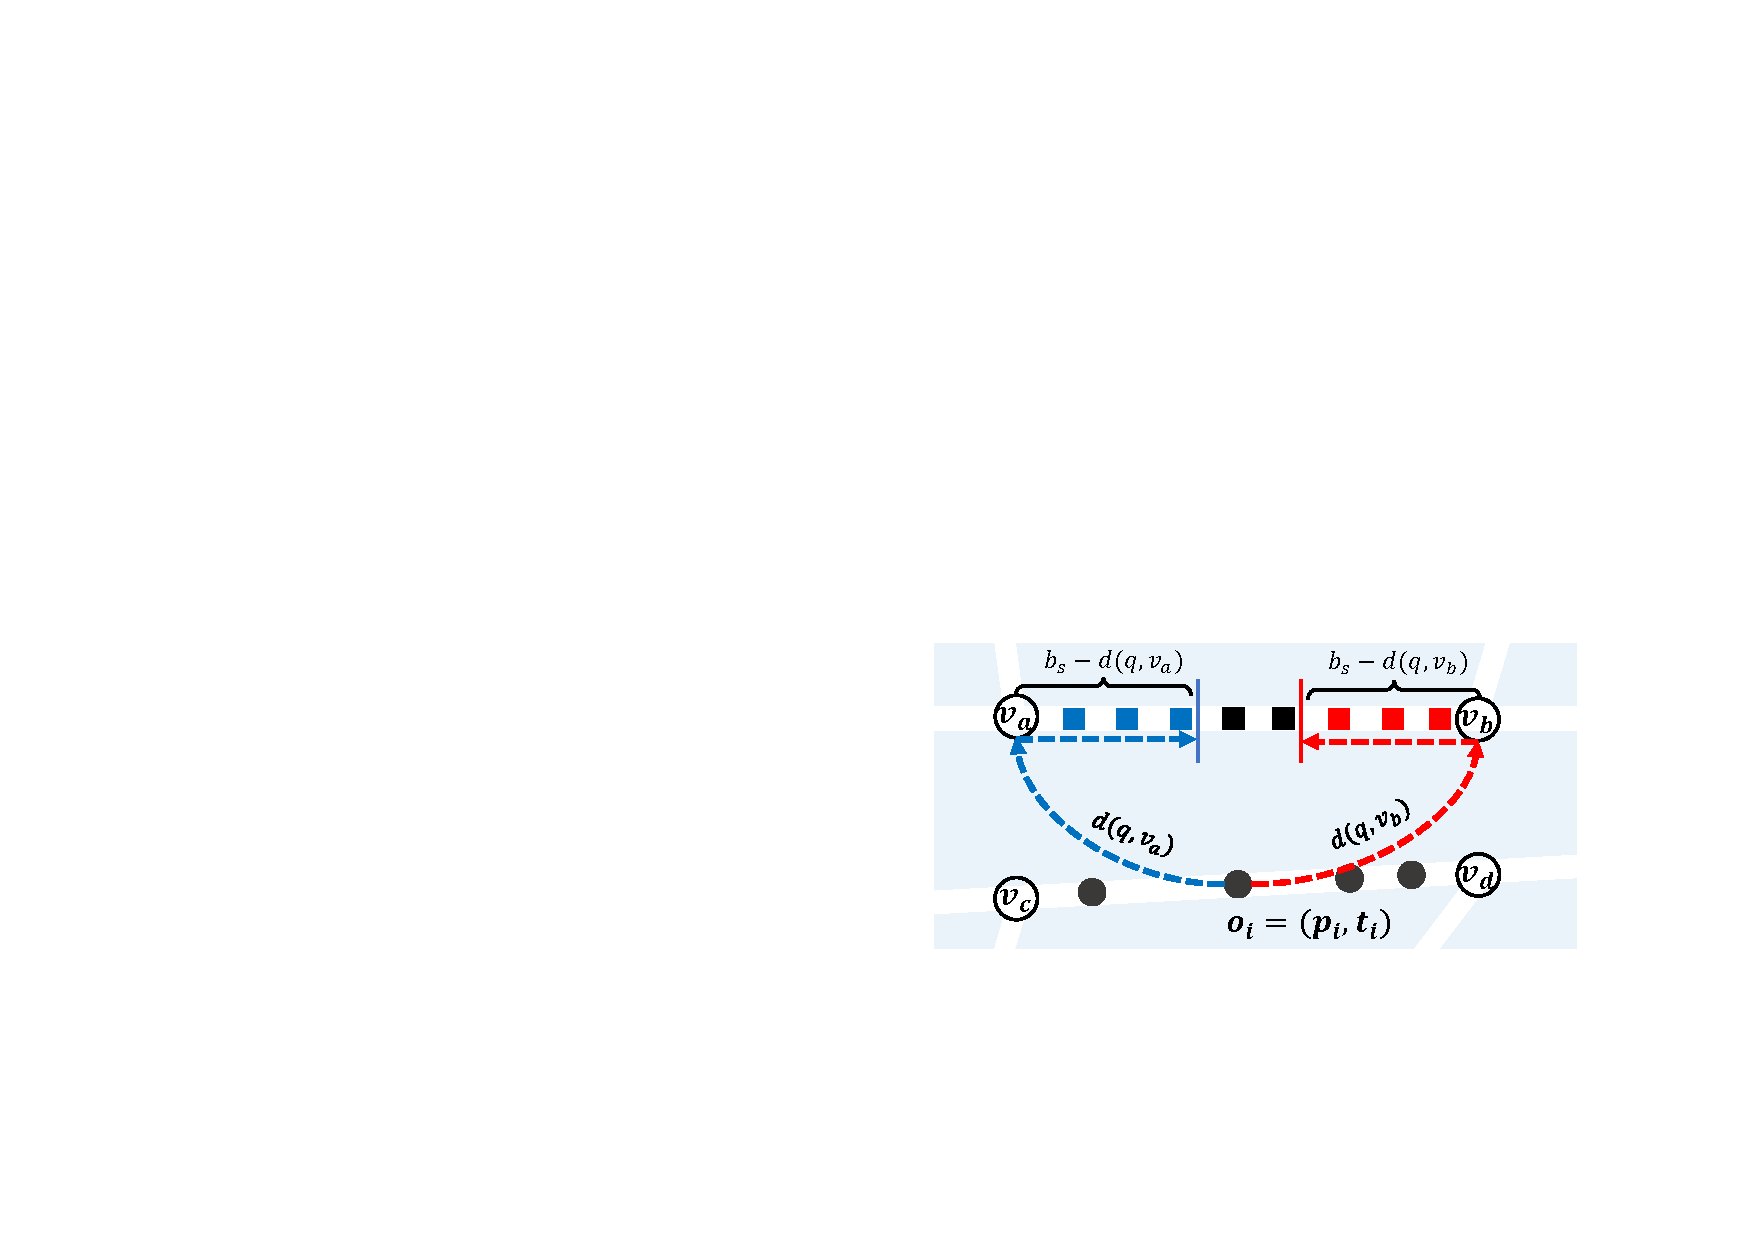
\includegraphics{../figures/Preliminary_LION.pdf}}
% 	\caption{The illustration of the LION method.}
% \end{figure}

% If the distance from a lixel $q$ to $v_a$, which is $d(q, v_a)$, is shorter than $b_s - d(p_i, v_a)$, this event $o_i$ will contribute to this lixel, i.e., updating the aggregation vector $\mathbf{L}$. So we can use $b_s - d(p_i, v_a)$ to find the boundary, i.e., the largest index $l$ that $d(v_a, q_l) \le b_s - d(p_i, v_a)$. Note all lixels are equidistant and $l$ can be computed in $O(1)$ instead of a binary search. Observing that this updating operation adds the same value from $\mathbf{L}_1$ to $\mathbf{L}_l$, we can easily record a delta value only at $\mathbf{L}_l$ and recover the result by adding up reversely.

% The other side for $v_b$ is similar and the index order is reversed. Besides, two influenced ranges also might be overlapped, so the extra breakpoint boundary $d(v_a, q_l) \le \frac{- d(p_i, v_a) + d(p_i, v_b) + d(v_a, v_b)}{2}$ is required.


% \begin{lemma}
% 	The time complexity of ADA and LION is $O(\vert E \vert T_{sp} + L\vert E \vert \log(\frac{N}{\vert E \vert}))$ and $O(\vert E \vert T_{sp} + N\vert E \vert + \vert E \vert ^2 + L)$, respectively. The space complexity is both $O(\vert V \vert + \vert E \vert + N + L + S_{sp})$.
% \end{lemma}







\subsection{算法框架}
\label{sec3.3:framework}

TN-KDE问题相比之下更加复杂,由于额外加入时间维度,数据点的聚合集分类会更加复杂。具体来说,时间维度上的距离是$\vert t - t_i \vert$,由于表达式中的绝对值函数,我们无法直接对这个表达式进行聚合,而是需要先分为$t_i < t$ 和 $t_i \ge t$分类计算。例如,对于更靠近 $v_c$ 且 $t_i < t$ 的聚合集,假设空间和时间核函数均采用三角核函数,对应的核密度计算公式会扩展为如下形式:

\begin{align}
	\label{eq:aggregate}
	&F_\Gamma(q) \notag \\
	=& \sum_{o_i \in O_\Gamma}
	\left(1 - \frac{d(q,p_i)}{b_s}\right)
	\left(1 - \frac{\vert t - t_i \vert}{b_t}\right) \notag \\
	=& \sum_{o_i \in O_\Gamma}
	\left(1-\frac{d(q, v_c) + d(v_c, p_i)}{b_s}\right)
	\left(1-\frac{t - t_i}{b_t}\right) \\
	=& \frac{1}{b_sb_t} \cdot 
	\begin{bmatrix}
		-1 \\
		b_s-d(q, v_c) \\
		-(b_t-t) \\
		(b_s-d(q, v_c))(b_t-t) \\
	\end{bmatrix}^\top \cdot
	\begin{bmatrix}
		\sum_{o_i \in O_\Gamma} d(v_c,p_i)t_i \\
		\sum_{o_i \in O_\Gamma} d(v_c,p_i) \\
		\sum_{o_i \in O_\Gamma} t_i \\
		\vert O_\Gamma \vert 
	\end{bmatrix} \notag
\end{align}

虽然核密度的计算额外增加了一个维度,但是依然可以拆解为两个向量。同理,第一个查询向量$\mathbf{Q}$仅和线段点 $q$ 有关,第二个聚合向量$\mathbf{A}$是聚合集中的所有数据点的属性值相加。
算法~\ref{algo:framework}描述了解决TN-KDE问题的主要框架。对于一个线段点 $q$,遍历每一条边 $e$上的所有聚合集$\Gamma$,并获取查询向量$\mathbf{Q}$和$\mathbf{A}$,即可计算$\Gamma$对核密度的贡献$F_\Gamma(q)$。将这些核密度累加起来,即可得到结果线段点 $q$ 上的核密度 $F(q)$。

\begin{algorithm}[h]
	\caption{TN-KDE问题框架}
	\label{algo:framework}
	\DontPrintSemicolon
	\SetKwComment{comment}{$\triangleright$ }{}
	
	\For{each lixel $q$ }{
		\For{each edge $e=(v_c, v_d) \in E$}{
			Get shared shortest path $d(q, v_c)$ and $d(q, v_d)$ \\
			\For{each aggregation $\Gamma$ on edge $e$}{
				$\mathbf{Q} \leftarrow$ the query vector 
				% \comment*{first vector in  Eq.{(\ref{eq:aggregate})}}

				$\mathbf{A} \leftarrow$ the aggregated vector
				% \comment*{second vector in Eq.{(\ref{eq:aggregate})}}

				$F_{\Gamma}(q) \leftarrow \mathbf{Q} \cdot \mathbf{A}$ \\
				$F_e(q) \leftarrow F_e(q) + F_{\Gamma}(q)$
			}
		}
		$F(q) \leftarrow F(q) + F_e(q)$
	}
\end{algorithm}

该框架和ADA算法类似,主要的难点在于如何高效地获取聚合向量$\mathbf{A}$~(算法\ref{algo:framework}第4行)。ADA算法只需简单的二分搜索即可获得聚合集及对应的聚合向量,但该方法无法简单扩展至高维空间,即在TN-KDE问题中,时间维度的加入使得数据点和聚合集的维护变得复杂。在下一章中,我们将探讨对每条边的数据点建立高效的索引,以维护这些聚合集而不增加额外的时间复杂度。